\documentclass{report}
\title{Susquehanna User Manual - v0.1.2 Milford}
\author{thetacola}
\usepackage{graphicx}
\usepackage{indentfirst}
\usepackage{wrapfig}
\usepackage{tcolorbox}
\pagenumbering{arabic}

\begin{document}
	\begin{figure}
		\centering
		
\includegraphics[width=0.7\linewidth]{img/logo}
	\end{figure}
	\maketitle
	\tableofcontents
	\chapter{Introduction}
	Susquehanna is a program made for the creation and management of conlangs. This application may also find use as a tool for the documentation of natural languages. The layout of Susquehanna is like a book, where content appears in the middle on pages (both left and right), with binder tabs on the left side to help with navigation. To the right of the tabs are tools for editing your language.
	\section{Tabs}
	\begin{wrapfigure}{r}{0.5\textwidth}
		\centering
		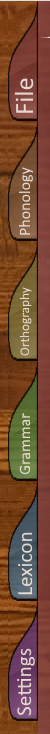
\includegraphics[width=0.038\textwidth]{img/tabs-screenshot}
		\caption{The six tabs in Susquehanna.}
		\label{fig:tabs-screenshot}
	\end{wrapfigure}
	Tabs can be found on the leftmost edge of the application whenever it is open. These tabs categorize tools into categories,	so that each tool is easier to find. These tabs are also color coded, and the color of the book background is decided by the currently selected tab. To check which tab is being used, the user can see which color book background matches which color tab.
	\par
	There are six tabs, those being File, Phonology, Orthography, Grammar, Lexicon, and Settings. This manual covers each tab in detail, for more information on each tab please check the table of contents to find the page about a given tab. When using Susquehanna on low-resolution displays or small window sizes, the tabs can be scrolled through using the scroll wheel. Using the PgUp and PgDown keys on the number pad also works. 
	\par
	\begin{tcolorbox}
	\textsc{For developers:} Adding a new tab to Susquehanna is fairly simple. This can be done by editing \emph{net.oijon.susquehanna.gui.Navbox}. First, create an image for your new tab. A template for this can be found in \emph{src/main/resources/img}. Save your image as \emph{\{name\}-tab.png}. Then, add a new BinderTab instance in the Navbox class, next to the rest of the BinderTab instances. Make sure to set the name of the tab to the name you picked earlier for the image, minus the "-tab.png" bit. Otherwise, your image will be unable to link to this tab. Then, edit the line starting with "VBox navVBox" in \emph{Navbox.Navbox()}, and add your tab to the end of the list. To make this tab functional, add \emph{\{tab variable name\}.createTransferAction(\{book ID\})} to \emph{Navbox.createTransferActions()}. Once these steps are done, you should have a fully functional tab.
	\par
	There is no limit set for the amount of tabs that can be loaded at a given time by Susquehanna, however performance and general usability will be impacted when adding several hundreds of tab. Furthermore, as JavaFX parents can "only" contain \emph{Integer.MAX\_VALUE} (around \(2^{31}\)) children, there's likely a limit of around \(2^{31}\) tabs. It should be noted that Susquehanna is not built to handle this many tabs, and would likely crash from the amount of images needed to render before this point (each tab image following the template is around 2.81kB, \(2.81 * 2^{31} \approx 6,034,429,051kB \approx\) 6TB, and the JVM is not happy handling anything more than 4TiB of memory at a given time). Scrolling through this amount of tabs trying to find the correct one would also likely not be a pleasant experience for the user, so tabs should be kept to a rather low amount if possible.
	\par
	More information on book IDs can be found later in the Tools section.
	\end{tcolorbox}
	\newpage
	\section{Tools}
	\begin{wrapfigure}{r}{0.5\textwidth}
		\centering
		
\includegraphics[width=0.2\textwidth]{img/info}
		\caption{An example of a tool button. This is the Info button, under the File tab.}
		\label{fig:tool-button}
	\end{wrapfigure}
	Tools are various pages that allow for the editing of a language. These take the form of buttons to the right of tabs. Each tab has a different set of tools corresponding to its category. For example, the phonology tab has the "View Phonology" and "Edit Phonology" tools, while the file tab has the "Info" and "Report Bug" tools. The page each tool takes the user to is also called a book. These tools are the main way different views are switched between in Susquehanna.
	
	\chapter{The File Tab}
	The first tab a user will encounter when first starting up Susquehanna is the file tab. This tab is responsible
	for things such as selecting a language, seeing debug information, and sending bug reports. In short, the file tab
	allows the user to change what is being worked on, and report when anything goes wrong.
	\section{New Language}
	\section{Open Language}
	\section{Info}
	\section{Report Bug}
	
	\chapter{The Phonology Tab}
	\section{View Phonology}
	\section{Edit Phonology}
	\section{Phonotactics}
	
	\chapter{The Orthography Tab}
	\section{View Orthography}
	\section{Edit Orthography}
	\section{Script}
	
	\chapter{The Grammar Tab}
	The grammar tab is a placeholder tab for a planned update. Currently, the grammar tab
	does not contain any usable tools.
	
	\chapter{The Lexicon Tab}
	\section{View Words}
	\section{Edit Words}
	
	\chapter{The Settings Tab}
	Like the grammar tab, the settings tab is a placeholder for a planned update. Currently,
	the settings tab does not contain any usable tools.
	
\end{document}